\setchapterstyle{kao}
\setchapterpreamble[u]{\margintoc}
\chapter{Contrasting distinct structured views to learn sentence embeddings}
% using a generative objective
\labch{structure-scale}

% \section{Training efficient sentence embedding models using structured encoders}
% \labsec{structure-scale}

\cleanchapterquote{When people say AI has “learned x” what they usually mean is that a deep learning model has learned a dataset well enough to find the pattern you asked for. It has no symbolic or logical abstraction. It is kahnemann system 1. It looks smart. It isn’t.}{Mark Madsen}{Twitter post, 2019}

% The previous sections proposed to train sentence encoders at scale, In \refch{1B} by augmenting the pre-training corpus size and in \refch{generative} by proposing alternative pre-training objectives. In this section, we focus on the encoder architecture. We train various encoders and combine them in an original multi-view setup.

%\bcomment{move after chap 5?}{}

% \section{Motivation}
% \labsec{structure:motivation}

% Inspired from linguistic insights, I assume structure is crucial to building consistent representations. I indeed expect sentence meaning to be a function of both syntax and semantic aspects. 
We hypothesize that structure is a crucial element to perform compositional knowledge. In particular, the heterogeneity of performances across models and tasks makes us assume that some structures may be better adapted for a given example or task. Therefore, combining diverse structures should be more robust for tasks requiring complex word composition to derive their meaning. Hence, we aim to evaluate the potential benefit from interactions between pairs of encoders. In particular, we propose a training method for which distinct encoders are learned jointly. We conjecture this association might improve our embeddings' power of generalization and propose an experimental setup to test our hypothesis.

We take inspiration from multi-view learning, which is successfully applied in a variety of domains. In such a framework, the model learns representations by aligning separate observations of the same object. Such observations are referred to as \textit{views}. In our case, we consider a view for a given sentence as the association of the plain sentence with several kinds of syntactic representations. 

Combining different structural views has already been proven to be successful in many NLP applications. \textcite{kong_11} provide a heuristic to combine dependency and constituency analysis for coreference resolution. \textcite{zhou_16, ahmed_19_2} combine Tree LSTM and standard sequential LSTM with a cross-attention method and observe improvements on a semantic textual similarity task. \textcite{chen_liu_17} combine CNN and Tree LSTM using attention methods and outperform both models taken separately on a sentiment classification task. Finally, \textcite{chen_17} combine sequential LSTM and Tree LSTM for natural language inference tasks. 

The novelty here is to combine distinct structured models to build standalone sentence embeddings, which has not yet been explored. This paradigm benefits from several structural advantages. It pairs nicely with contrastive learning, as already mentioned. It may thus be trained in a self-supervised manner that does not require data annotation. Moreover, our method is not specific to a certain kind of encoder architecture, and it does not require, for example, the use of attention layers or tree-structured models.

Our setup could therefore be extended with any encoding function. Finally, our training method induces an interaction between models during inference and, paramountly, during the training phase.

We organize our section as follows: \refsec{structure:method} reviews the contrastive and multi-view training method we used. In \refsec{structure:experiments}, we present our training and evaluation setup. We then propose an in-depth analysis of our results.

\section{Method}
\labsec{structure:method}

\subsection{Contrastive learning}

\begin{figure*}[!htb]
\begin{center}
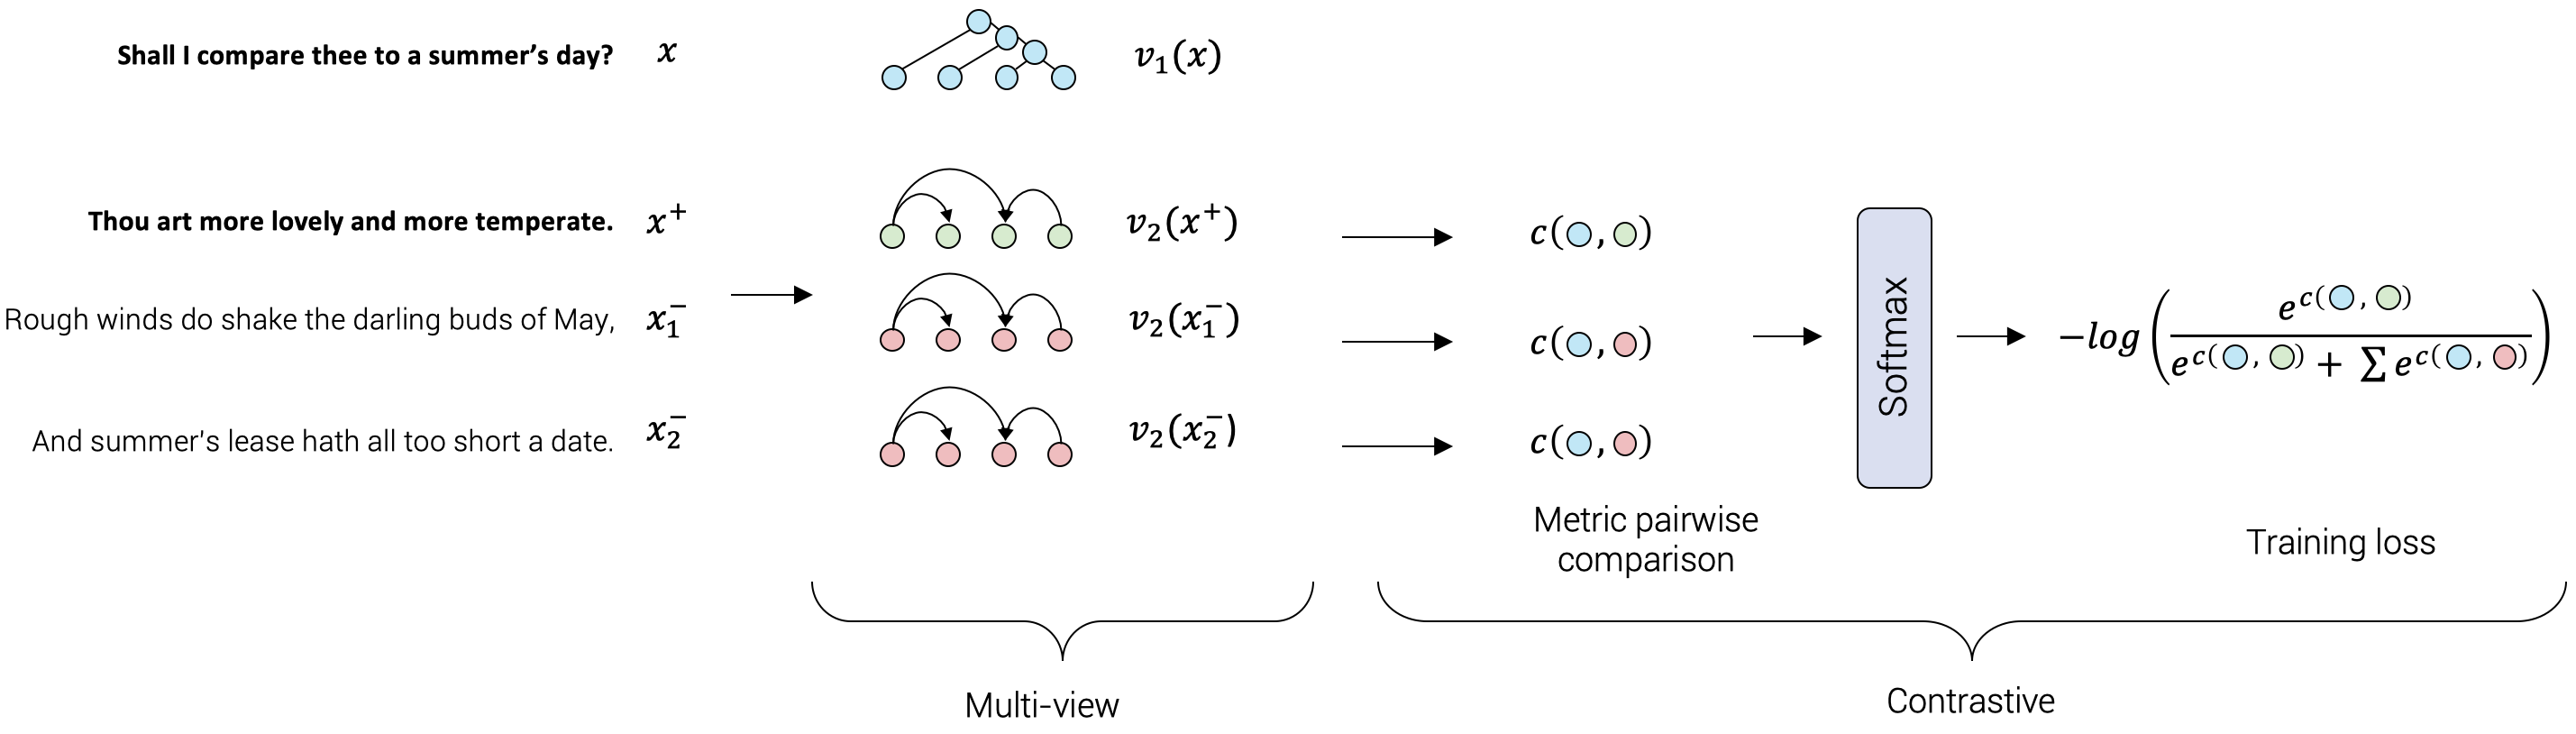
\includegraphics[width=15cm]{images/contrastive-4.png}
\end{center}
\caption{Contrastive training method. The objective is to reconstruct the storyline. Sentences are presented in their original order. Given an anchor sentence $x$, the model has to identify the context sentence $x^+$ out of negative samples $x_1^-, x_2^-$. Sentences are encoded using separate views, which are composed within a pairwise distance matrix. }
\labfig{structure:contrastive}
\end{figure*}

We train our model using the contrastive objective from \textcite{logeswaran_18}, detailed in \refsec{training}. The method takes inspiration from the distributional hypothesis successfully applied for words, but this time, to identify context sentences. Given a sentence $s$, a corresponding context sentence $s^+$ and a set of $K$ negative samples $s^-_1 \cdots s^-_K$, the training objective is to maximize the probability of predicting the correct sentence among negative samples: $p(s^+ | S)$ with $S = \{s, s^+, s^-_1 \cdots s^-_K\}$. As illustrated in \reffig{structure:contrastive}, two sentences encoders $f$ and $g$ are defined and the conditional probability is estimated as follow:

\[
p(s^+ | S) = \frac{e^{c\left(f(s), g(s^+)\right)}}{e^{c\left(f(s), g(s^+)\right)}+\sum_{i=1}^Ne^{c\left(f(s), g(s^-_i)\right)}}
\]

With $c(x, y)$ the scoring function. \textcite{logeswaran_18} simply use an inner product for $c$ such as $c\left(x, y\right) = x^Ty$. In our case, as the encoders $f$ and $g$ have distinct architectures. To prevent the case of $f$ and $g$ having distinct norms and the inner product resulting in irrelevant information, we choose a bilinear function defined as $c\left(x, y\right) = x^TWy$ \parencite{tschannen_20}. At inference time, the sentence representation is obtained as the concatenation of the two encoders $f$ and $g$ such as $s \rightarrow [f(s);g(s)]$, as illustrated in \reffig{inference}. In \textcite{logeswaran_18}, $f$ and $g$ use the same RNN encoder. However, the authors observe that the encoders might learn redundant features. To limit this effect, they propose to use a distinct set of embeddings for each encoder. 

We propose addressing this aspect by enhancing the method with a multi-view framework and using a distinct structured model for the encoders $f$ and $g$. We hypothesize that some structures may be better adapted for a given example or task. 
For example, dependency parsing usually sets the verb as the root node. Whereas in constituency parsing, subject and verb are often split between the left and right sub-trees from the root node (as illustrated in \reffig{multi-views}). Therefore, the combination of different structures should be more robust for tasks requiring complex word composition and be less sensitive to lexical variations. Consequently, we propose a training procedure that allows the model to benefit from the interaction of various syntactic structures.
%the \bcomment{right and left child}{not obvious to me}
\subsection{Language views}

Multi-view aims at learning representations from data represented by multiple independent sets of features. We generalize the notion of view for a sentence as the application of a specific syntactic framework. For each view, we use an \textit{ad-hoc} algorithm that maps the structured sentence into an embedding space.

We consider structures exposed in \refsec{survey:encoding}: Vanilla GRU (\textsc{Seq}), dependency tree combined with an attentive Child-Sum Tree LSTM (\textsc{Dep}), Constituency tree combined with N-Ary Tree LSTM (\textsc{Const}).\sidenote{We introduced this attentive version of the Child-Sum Tree LSTM for which details are given in \refsec{architectures:tree}} Although under some hypotheses equivalences might be derived between the last two representations schemes, we hypothesize that, in our context, the corresponding sequence of operations might provide the possibility of capturing rather distinct linguistic properties. The various models may, therefore, be complementary and their combination allows for more fine-grained analysis. 

For the \textsc{Dep} view, the dependency tree is obtained using the deep biaffine parser from \textcite{dozat_17}. We used an open-source implementation of the parser and replaced the pos-tag features with features obtained with \bert.\sidenote{\url{https://github.com/yzhangcs/biaffine-parser}} Therefore we do not need pos-tags annotations to parse our corpus. 

For the \textsc{Const} view, the structure is obtained using the constituency neural parser from \textcite{klein_18}. We binarize the trees to ensure that every node has exactly two dependents. The binarization is performed using a left markovization \parencite{klein_2003} and unary productions are collapsed in a single node. Regarding the inference speed, the constituency parser is the bottleneck and parses around 500 sentences/second. In our case, the parsing of the entire corpus (40M sentences) takes about a day to complete.

\begin{figure}[!htb]
\begin{center}
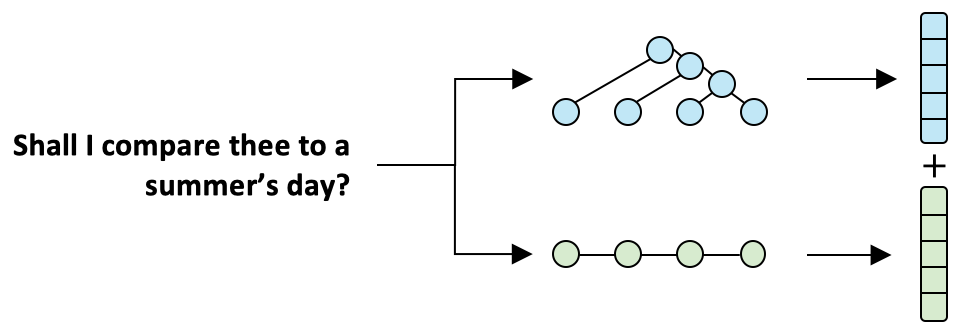
\includegraphics[width=10cm]{images/contrastive-inf.png}
\end{center}
\caption{Multi-view sentence embedding. At inference, embeddings are the concatenation from both views.}
\labfig{inference}
\end{figure}

\section{Experiments}
\labsec{structure:experiments}

We train our models on the UMBC dataset \parencite{han_13}.\sidenote{The bookcorpus introduced in \textcite{zhu_15} and traditionally used for sentence embedding is no longer distributed for copyright reasons. Therefore, we prefer a corpus freely available. The impact of the training dataset choice is analyzed in \refsec{impact-corpus}.}\footnote{\url{https://ebiquity.umbc.edu/blogger/2013/05/01/umbc-webbase-corpus-of-3b-english-words/}} We limit our corpus to the first 40M sentences from the tokenized corpus. Indeed, \textcite{logeswaran_18} already analyzed the effect of the corpus size, and we focus here on the impact of our multi-view setting. For each sample, we train the model to maximize the probability of predicting the correct sample among negative samples. In practice, we constitute mini-batches of consecutive sentences. For each sentence in the mini-batch, the correct samples correspond to context sentences, that is, sentences immediately after and before the target sentence. Other sentences in the batch are considered negative examples. We use a batch size of 400. Therefore, for each target sentence, we consider 2 positive samples and 397 negative samples. Model hyper parameters are fixed given literature on comparable work \parencite{tai_15, logeswaran_18}. All models are trained using the Adam optimizer with a $5e^{-4}$ learning rate. Regarding the infrastructure, we use a Nvidia GTX 1080 Ti GPU. All model weights are initialized with a Xavier distribution and biases set to 0. We do not apply any dropout. 

For the vocabulary, we follow the setup proposed in \textcite{kiros_15, logeswaran_18} and we train two models in each configuration. One initialized with pre-trained embedding vectors. The vectors are not updated during training and the vocabulary includes the top 2M cased words from the 300-dimensional GloVe vectors \parencite{pennington_14}.\sidenote{\url{https://nlp.stanford.edu/projects/glove/}} The other is limited to 50K words initialized with a Xavier distribution and updated during training. For inference, the vocabulary is expanded to 2M words using a linear projection.

\subsection{Evaluation on SentEval}

\begin{table*}[!htb]
\footnotesize
% \begin{minipage}{\textwidth}
\centering {
\begin{tabularx}{16cm}{@{}c c Y | Y Y Y Y Y Y Y Y Y Y @{}}
\toprule
\multirow{2}{*}{\textbf{Model}} & \multirow{2}{*}{\textbf{Dim}} & \multirow{2}{*}{\textbf{Hrs}} & \multirow{2}{*}{\textbf{MR}} & \multirow{2}{*}{\textbf{CR}} & \multirow{2}{*}{\textbf{SUBJ}} & \multirow{2}{*}{\textbf{MPQA}} & \multirow{2}{*}{\textbf{TREC}} &  \multicolumn{2}{c}{\textbf{MRPC}} &  \multicolumn{3}{c}{\textbf{SICK-R}}\\%\cmidrule(r){9-10} \cmidrule(r){11-13}
 &  &  &  &  &  &  &  & \textbf{Acc} & \textbf{F1} & \textbf{$r$} & \textbf{$\rho$} & \textbf{MSE}\\\midrule
\multicolumn{13}{c}{\textit{Context sentences prediction}} \\\midrule
FastSent & $\leq$\numprint{500} & 2 & 70.8 & 78.4 & 88.7 & 80.6 & 76.8 & 72.2 & 80.3 & --- & --- & ---\\
FastSent + AE & $\leq$\numprint{500} & 2 & 71.8 & 76.7 & 88.8 & 81.5 & 80.4 & 71.2 & 79.1 & --- & --- & ---\\
Skipthought & \numprint{4800} & 336 & 76.5 & 80.1 & 93.6 & 87.1 & 92.2 & 73.0 & 82.0 & 85.8 & 79.2 & 26.9\\
Skipthought + LN & \numprint{4800} & 672 & 79.4 & 83.1 & 93.7 & 89.3 & --- & --- & --- & 85.8 & 78.8 & 27.0\\
Quickthought & \numprint{4800} & 11 & \textbf{80.4} & \textbf{85.2} & \textbf{93.9} & \textbf{89.4} & \textbf{92.8} & \textbf{76.9} & \textbf{84.0} & \textbf{86.8} & \textbf{80.1} & \textbf{25.6}\\
\midrule\multicolumn{13}{c}{\textit{Sentence relations prediction}} \\\midrule
InferSent & \numprint{4096} & --- & \textbf{81.1} & \textbf{86.3} & 92.4 & 90.2 & 88.2 & \textbf{76.2} & \textbf{83.1} & \textbf{\underline{88.4}} & --- & ---\\
DisSent Books 5 & \numprint{4096} & --- & 80.2 & 85.4 & 93.2 & 90.2 & 91.2 & 76.1 & --- & 84.5 & --- & ---\\
DisSent Books 8 & \numprint{4096} & --- & 79.8 & 85.0 & \textbf{93.4} & \textbf{\underline{90.5}} & \textbf{\underline{93.0}} & 76.1 & --- & 85.4 & --- & ---\\
\midrule\multicolumn{13}{c}{\textit{Pre-trained transformers}} \\\midrule
\textsc{Bert}-base [CLS] & \numprint{768} & 96 & 78.7 & 84.9 & 94.2 & 88.2 & \textbf{91.4} & 71.1 & --- & 75.7$^\dagger$ & --- & ---\\
\textsc{Bert}-base [NLI] & \numprint{768} & 96 & \textbf{\underline{83.6}} & \textbf{\underline{89.4}} & \textbf{94.4} & \textbf{89.9} & 89.6 & \textbf{76.0} & --- & \textbf{84.4}$^\dagger$ & --- & ---\\
\midrule\multicolumn{13}{c}{\textit{\textbf{Our models (GloVe \& Pretrained Embeddings)}}} \\\midrule
\textsc{Seq}, \textsc{Const}$^\dagger$ & \numprint{4800} & 41 & 79.8 & 82.9 & 94.6 & 88.5 & 90.4 & 76.4 & 83.7 & 86.1 & 78.9 & 26.3\\
\textsc{Dep}, \textsc{Seq}$^\dagger$ & \numprint{4800} & 27 & 79.7 & 82.2 & 94.4 & 88.6 & 91.0 & \textbf{\underline{77.9}} & \textbf{\underline{84.4}} & 86.6 & 79.8 & 25.5\\
\textsc{Dep}, \textsc{Const}$^\dagger$ & \numprint{4800} & 39 & \textbf{80.7} & \textbf{83.6} & \textbf{\underline{94.9}} & \textbf{89.2} & \textbf{92.6} & 76.8 & 83.6 & \textbf{87.0} & \textbf{\underline{80.3}} & \textbf{\underline{24.8}}\\
\bottomrule
\end{tabularx}}
\caption{SentEval Task Results Using Fixed Sentence Encoder. 
We divided the table into sections. The first range of models is directly comparable to our model as the training objective is to identify context sentences. The second section objective is to identify the correct relationship between a pair of sentences. The third section reports pre-trained transformer-based models. The last section reports the results from our models. FastSent is reported from \textcite{hill_16}. Skipthoughts results from \textcite{kiros_15} Skipthoughts + LN which includes layer normalization method from \textcite{ba_16}. We considered the Quickthought results \cite{logeswaran_18} with a pre-training on the bookcorpus dataset. DisSent and Infersent are reported from \textcite{nie_19} and \textcite{conneau_17} respectively. Pre-trained transformers results are reported from \textcite{reimers_19}. The \textbf{Hrs} column indicates indicative training time, the \textbf{Dim} column corresponds to the sentence embedding dimension. $^\dagger$\, indicates models that we had to re-train. Best results in each section are shown in \textbf{bold}, best results overall are \underline{underlined}. Performance for \textbf{SICK-R} results are reported by convention as $\rho \text{ and } r \times 100$. In all columns, higher scores indicate better performance, with the exception of the MSE, in which lower results indicate better performance}
\labtab{contrastive-soa}
\end{table*}

As is usual for models aiming to build generic sentence embeddings \parencite{kiros_15, hill_16, arora_17, conneau_17, logeswaran_18, nie_19}, we use tasks from the SentEval benchmark \parencite{conneau_18}.\sidenote{Senteval is posterior to most of the references. However, these studies do evaluate on tasks later included in the benchmark.} SentEval is specifically designed to assess the quality of the embeddings themselves rather than the quality of a model specifically targeting a downstream task, as is the case for the GLUE and SuperGLUE benchmarks \parencite{wang_19_glue, wang_19_superglue}. Indeed, the evaluation protocol prevents fine-tuning the model during inference and the architecture to tackle the downstream tasks is kept minimal. Moreover, the embedding is kept identical for all tasks, thus assessing their properties of generalization. 

Therefore, classification tasks from the SentEval benchmark are usually used for evaluation of sentence representations \parencite{conneau_18}: the tasks (presented in \refsec{survey:downstream}) include sentiment and subjectivity analysis (\textbf{MR, CR, SUBJ, MPQA}), question type classification (\textbf{TREC}), paraphrase identification (\textbf{MRPC}) and semantic relatedness (\textbf{SICK-R}). Contrasting the results of our model on this set of tasks will help to better understand its properties. MR, CR, SUBJ, MPQA tasks are binary classification tasks with no pre-defined train-test split. We therefore use a 10-fold cross validation. For the other tasks, we use the proposed train/dev/test splits. We give examples for each tasks in \reftab{senteval:examples}.
%We use either the pre-defined train/dev/test splits or perform a 10-fold cross-validation. 
We follow the linear evaluation protocol of \textcite{kiros_15}, where a logistic regression or softmax classifier is trained on top of sentence representations. The dev set is used to choose the regularization parameters and results are reported on the test set. 

The \textbf{MR, CR, SUBJ, MPQA} and \textbf{TREC} are classification tasks, for which we report the accuracy. For \textbf{MRPC}, we report the accuracy and f1 score. Finally, the \textbf{SICK-R} task is a regression task. We report the Pearson ($r$) and Spearman ($\rho$) correlations as well as the mean squared error (mse).

% \paragraph{Results analysis} 

We compare the properties of distinct views combination on downstream tasks. Results are compared with state-of-the-art methods in \reftab{contrastive-soa}. The first set of methods (\textsl{Context sentences prediction}) are trained to reconstruct the storyline of  books. % relies on a distributional hypothesis: models 
The second set of models (\textsl{Sentence relations prediction}) is pre-trained on a supervised task. Infersent \parencite{conneau_17} is trained on the SNLI dataset, which proposes to predict the entailment relation between two sentences. DisSent \parencite{nie_19} proposes a generalization of the method and builds a corpus of sentence pairs with more possible relations between them. Finally, we include models relying on transformer architectures (Pre-trained transformers) for comparison. In particular, \textsc{Bert}-base and \textsc{Bert}-base fine-tuned on the SNLI dataset \parencite{reimers_19}. 
In \reftab{contrastive-soa}, we observe that our models expressing a combination of views such as (\textsc{Dep}, \textsc{Seq}) or (\textsc{Dep}, \textbf{const}) give better results than the use of the same view (\textbf{seq}, \textbf{seq}) used in Quickthought model. It seems that the entanglement of views benefits the sentence embedding properties. In particular, we obtain state-of-the-art results for almost every metric from \textbf{MRPC} and \textbf{SICK-R} tasks, which focus on paraphrase identification. For the \textbf{MRPC} task, we gain a full point in accuracy and outperform \textsc{Bert} models. We hypothesize structure is important for achieving this task, especially as the dataset is composed of rather long sentences. The \textbf{SICK-R} dataset is structurally designed to discriminate models that rely on compositional operations. 

This also explains the score improvement on this task. Tasks such as \textbf{MR}, \textbf{CR} or \textbf{MPQA} consist in sentiment or subjectivity analysis. We hypothesize that our models are less relevant in this case: such tasks are less sensitive to structure and depend more on individual word or lexical variation.

\subsection{Impact of the multi-view}
\labsec{impact-multi-view}

We aim to measure the impact of multi-view specifically. Table~\ref{table:multi-view} compares all possible view pairs out of \textsc{Dep}, \textsc{Const} and \textsc{Seq} views. For each multi-view model, we report the average score from SentEval tasks.\sidenote{We scale all metrics as percentages. In particular, we use 100 - MSE for the \textbf{SICK-R} task. The final score corresponds to the average of all tasks. We average the scores for tasks with multiple metrics (\textbf{MRPC} and \textbf{SICK-R}).} The first section of the Table corresponds to \textit{single-view} models, for which both views from the pair are identical. The second section reports multi-view models. 

Multi-view models outperform those using a single view. Given our experiment, it is advantageous to use multiple views instead of one. It also confirms our hypothesis that combining multiple structured models or views yields richer sentence embeddings.

\begin{table}[!htb]
\footnotesize
% \begin{minipage}{\textwidth}
\centering {
\begin{tabularx}{\textwidth}{@{}l c | Y@{}}
\toprule
\textbf{Model} & \textbf{Dim} & \textbf{Avg. SentEval Score} \\\midrule
\multicolumn{3}{c}{\textit{Single-view models}} \\\midrule
\textsc{Const}, \textsc{Const} & \numprint{4800} & 84.4\\
\textsc{Dep}, \textsc{Dep} & \numprint{4800} & 84.6\\
\textsc{Seq}, \textsc{Seq} & \numprint{4800} & 84.9\\\midrule
\multicolumn{3}{c}{\textit{Multi-view models}} \\\midrule
\textsc{Seq}, \textsc{Const} & \numprint{4800} & 85.1\\
\textsc{Seq}, \textsc{Dep} & \numprint{4800} & 85.3\\
\textsc{Dep}, \textsc{Const} & \numprint{4800} & \textbf{86.0}\\
\bottomrule
\end{tabularx}}
\caption{Impact of the multi-view. The first section corresponds to single-view setups for which $f$ and $g$ are the same views. The second section reports multi-view models. For each model, we report the average score on the SentEval benchmark.}
\label{table:multi-view}
\end{table}

\subsection{Qualitative results}

\begin{figure*}[htb!]
\centering
\begin{subfigure}[b]{8cm}
    \centering
    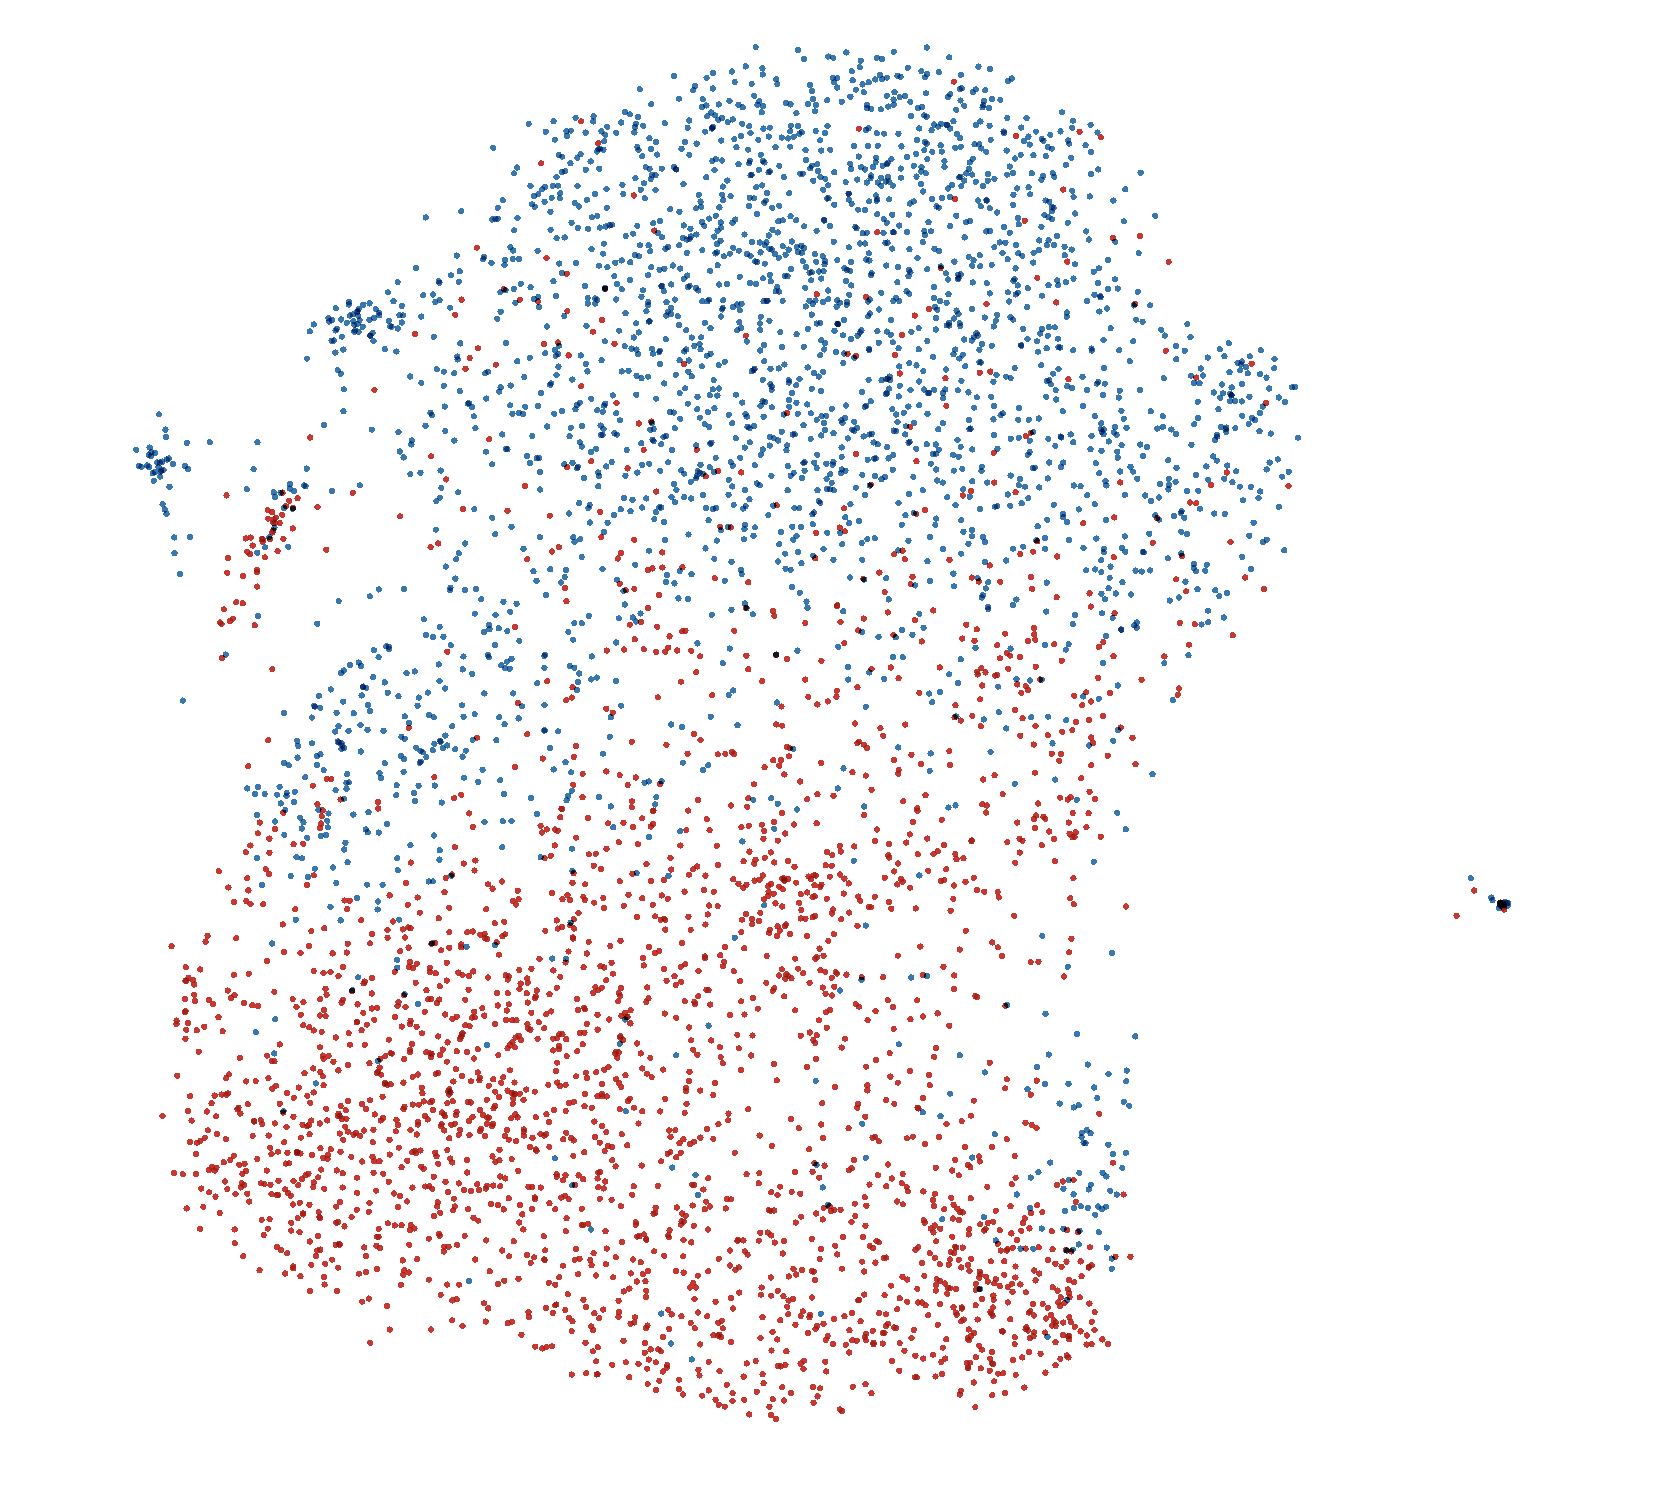
\includegraphics[width=7.5cm]{images/SUBJ_MV_DEP_CONST_no_sphere.png}
    \label{fig:sub1}
\end{subfigure}
\hfill
\begin{subfigure}[b]{8cm}  
    \centering 
    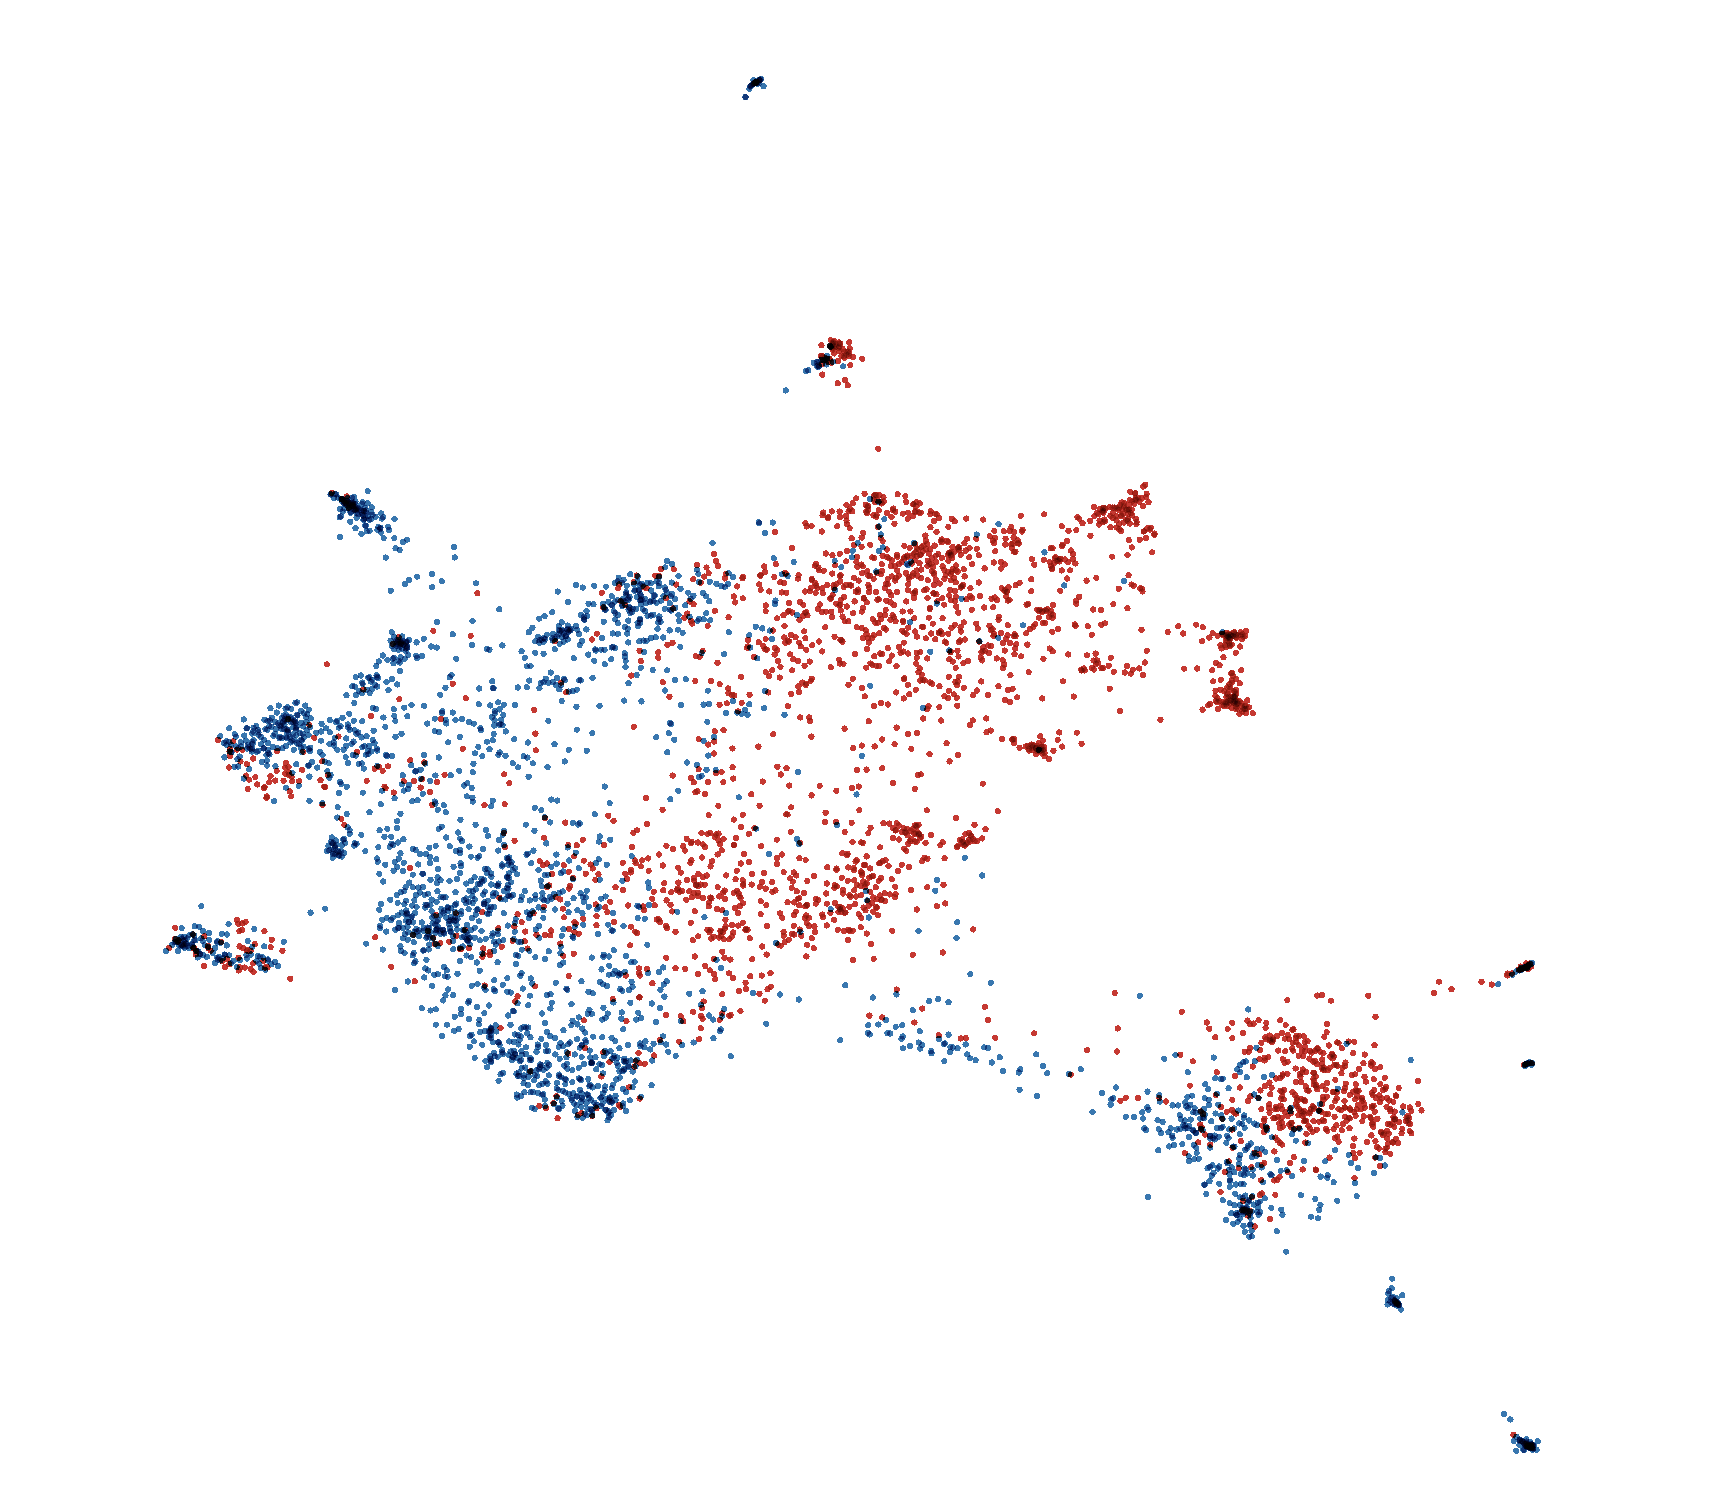
\includegraphics[width=7.5cm]{images/SUBJ_QT_no_sphere.png}
    \label{fig:sub2}
\end{subfigure}
\caption{Projection of the embeddings from the \textbf{SUBJ} task. \textit{(left)} The \dep, \const model is used (\textit{right}) We train a the Quickthought model using scripts from \parencite{logeswaran_18} on the UMBC dataset. Both dimension reductions are performed using the UMAP algorithm \parencite{mcinnes_18}. Points in \textcolor{blue}{blue} correspond to sentences with the label "objective". Points in \textcolor{red}{red} correspond to sentences with the label "subjective". In both cases, samples appear well separated given their labels.}
\labfig{subj:projection}
\end{figure*}
%  \bcomment{here we miss some critical information: what are the labels ? and to which color do they map. The plots have no legend at all }{}

We analyze the embeddings from a qualitative perspective and explore the sentences from the \textbf{SICK-R} test set. We retrieved the closest neighbors using cosine distance. We compare the results with the Quickthought model. We illustrate in \reftab{sts} a panel of examples presenting interesting linguistic properties. Models seem somehow robust to adjective expansions illustrated in the first examples. Indeed, the closest expression from \textit{"A black bird "} is \textit{"A bird , which is black"}. However, the second retrieved sentence is semantically correct for only the \const, \seq association. Quick-thought and \dep, \const present a weakness toward word scrambling for this specific example. We investigate passive forms in the second example. The \const, \seq and Quickthought models seem to attach too much weight to the sentence syntax rather than the semantic. This time the association of \dep and \const views retrieves  corresponding active sentences. Last but not least, we examine how models respond to the notion of scaling. Interestingly, Quickthought and \dep, \const are able to bring together "\textit{crowd}" and "\textit{group}" notions.

From a graphic perspective, we projected in two dimensions the sentences from the \textbf{SUBJ} task, for which we obtained state-of-the-art results. We use the UMAP \parencite{mcinnes_18} algorithm for dimensionality reduction and compare our multi-view setup with the Quickthought model. The projection is illustrated in \reffig{subj:projection}. While the Figure does not reveal any critical distinction between models, samples appear well separated in both cases.

\begin{table*}[!htb]
\footnotesize
\centering {
\begin{tabularx}{16cm}{@{}llY}
\toprule
\textbf{Encoder} & \textbf{Query and two closest sentences} & \textbf{Cosine distance}\\
\midrule
\midrule
\multicolumn{3}{c}{\textit{A black bird is sitting on a dead tree}}\\
\midrule
\multirow{2}{*}{\dep{}, \const{}} & A bird , which is black , is sitting on a dead tree & 0.118\\
& A dead bird is near a black man sitting on a tree & 0.139 \\
\midrule
\multirow{2}{*}{\const{}, \seq{}} & A bird , which is black , is sitting on a dead tree & 0.118\\
& The black bird is sitting in a leafless tree & 0.143 \\
\midrule
\multirow{2}{*}{Quickthought} & A bird , which is black , is sitting on a dead tree & 0.172\\
& A dead bird is near a black man sitting on a tree & 0.172 \\
\midrule
\multicolumn{3}{c}{\textit{Rugby is being played by some men}}\\
\midrule
\multirow{2}{*}{\dep{}, \const{}} & Rugby players are tackling each other & 0.381\\
& Some men are playing rugby & 0.392 \\
\midrule
\multirow{2}{*}{\const{}, \seq{}} & Guitar is being played by two men & 0.401\\
& Rugby players are tackling each other & 0.403 \\
\midrule
\multirow{2}{*}{Quickthought} & Guitar is being played by two men & 0.455\\
& Rugby players are tackling each other & 0.462 \\
\midrule
\multicolumn{3}{c}{\textit{A crowd of people is near the water}}\\
\midrule
\multirow{2}{*}{\dep{}, \const{}} & A crowd of people is far from the water & 0.079\\
& A group of people is near the ocean & 0.356 \\
\midrule
\multirow{2}{*}{\const{}, \seq{}} & A crowd of people is far from the water & 0.063\\
& A man is coming out of the water & 0.313 \\
\midrule
\multirow{2}{*}{Quickthought} & A crowd of people is far from the water & 0.067\\
& Two people are wading through the water & 0.388 \\
\bottomrule
\end{tabularx}}
\caption{A qualitative exploration of the sentence embedding space. We embed the sentences from the \textbf{SICK-R} test set. Given a query sentence, we retrieve the closest two sentences from the dataset using cosine distance. We compare the results of the semantic search using distinct views or single views combinations.}
\labtab{sts}
\end{table*}

\subsection{Impact of the corpus choice}
\labsec{impact-corpus}

We choose to make use of a distinct corpus as the BookCorpus dataset is no longer distributed for copyright reasons. We run QuickThought scripts \parencite{logeswaran_18} using our dataset based on the UMBC corpus to compare both setups. Results are detailed in the first section from \reftab{corpus} and are rather close in both configurations. Indeed, except for the \textbf{SUBJ} and \textbf{MR} task, the use of our dataset penalizes the results. Our corpus is indeed restricted to 40M sentences, in comparison with 74M for the Bookcorpus. Regarding the dataset size and the SentEval results, we have considered that the comparison holds.

\begin{table}[!htb]
\footnotesize
% \begin{minipage}{\textwidth}
\centering {
\begin{tabularx}{\textwidth}{@{}l c | Y@{}}
\toprule
\textbf{Model} & \textbf{Dim} & \textbf{Avg. SentEval Score} \\\midrule\midrule
\dep{}, \const{}$^\dagger$ (our model) & \numprint{4800} & 86.0 \\\midrule
 \multicolumn{3}{c}{\textit{Impact of the pretraining corpus on Quickthought}}\\\midrule
Quickthought (results from paper) & \numprint{4800} & 86.1 \\
Quickthought (UMCB 40M)$^\dagger$ & \numprint{4800} & 86.2 \\\midrule
 \multicolumn{3}{c}{\textit{Impact of the embedding size}} \\\midrule
\textsc{Bert}-base [CLS]$^\dagger$ & \numprint{768} & 78.2 \\
\textsc{Bert}-base [CLS] /w random projection$^\dagger$ & \numprint{4096} & 80.3 \\\midrule
 \multicolumn{3}{c}{\textit{Impact of pre-training}} \\\midrule
Rand$^\dagger$ & \numprint{4096} & 45.3 \\
Rand \textsc{BoW}$^\dagger$ & \numprint{4096} & 63.7 \\
Rand \textsc{LSTM} & \numprint{4096} & 83.4 \\
\bottomrule
\end{tabularx}}
\caption{\labtab{corpus}Study on SentEval task results. We first report our average score on the benchmark with our multi-view \dep{}, \const{} model. We compare distinct configurations with this reference to better qualify specific parameters' impact. The first section compares the impact of the training dataset for Quickthought. The following section focuses on the impact of the embedding size. To this end, hidden representations are projected into a larger embedding space using a random, fully connected layer. The final section compares an entirely random projection and a BoW or \textsc{LSTM} models randomly initialized with those pre-trained on our self-supervised task. $^\dagger$ indicates models that we train.}
\end{table}

% \begin{table*}[!htb]
% \footnotesize
% % \begin{minipage}{\textwidth}
% \centering {
% \begin{tabularx}{16cm}{@{}c| Y Y Y Y Y Y Y Y Y Y @{}}
% \toprule
% \multirow{2}{*}{\textbf{Model}} & \multirow{2}{*}{\textbf{MR}} & \multirow{2}{*}{\textbf{CR}} & \multirow{2}{*}{\textbf{SUBJ}} & \multirow{2}{*}{\textbf{MPQA}} & \multirow{2}{*}{\textbf{TREC}} &  \multicolumn{2}{c}{\textbf{MRPC}} &  \multicolumn{3}{c}{\textbf{SICK-R}}\\%\cmidrule(r){9-10} \cmidrule(r){11-13}
%  &  &  &  &  &  & \textbf{Acc} & \textbf{F1} & \textbf{$r$} & \textbf{$\rho$} & \textbf{MSE}\\\midrule
%  \multicolumn{11}{c}{\it Impact of the pretraining corpus on QuickThought} \\\midrule
% Quickthoughts (results from paper) & 80.4 & \textbf{85.2} & 93.9 & \textbf{89.4} & \textbf{92.8} & \textbf{76.9} & 84.0 & \textbf{86.8} & \textbf{80.1} & \textbf{25.6}\\
% Quickthoughts (UMCB 40M)$^\dagger$ & \textbf{80.9} & 84.4 & \textbf{95.1} & 88.9 & 92.2 & 75.8 & --- & 86.0 & --- & ---\\\midrule
%  \multicolumn{11}{c}{\it Impact of the embedding size} \\\midrule
% \textsc{Bert}-base [CLS] $^\dagger$& \textbf{77.3} & 81.3 & 92.7 & 85.0 & 80.2 & 69.9 & --- & 61.0 & --- & ---\\
% \textsc{Bert}-base [CLS] /w random projection $^\dagger$& 77.1 & \textbf{82.6} & \textbf{93.1} & \textbf{85.9} & \textbf{80.8} & \textbf{71.3} & --- & \textbf{71.0} & --- & ---\\\midrule
%  \multicolumn{11}{c}{\it Impact of pre-training}\\\midrule
% \dep{}, \const{}$^\dagger$ & \textbf{80.7} & \textbf{83.6} & \textbf{94.9} & \textbf{89.2} & \textbf{92.6} & \textbf{76.8} & \textbf{83.6} & \textbf{87.0} & \textbf{80.3} & \textbf{24.8}\\
% Rand \textsc{LSTM} & 77.2 & 78.7 & 91.9 & 87.9 & 86.5 & 74.1 & --- & 86.0 & --- & ---\\
% \bottomrule
% \end{tabularx}}
% \caption{\labtab{corpus}Study on SentEval task results: the first section compares the impact of the training dataset for QuickToughts. The next section focuses on the impact of the embedding size. To this end, hidden representations are projected into a larger embedding space using a random, fully connected layer. The final Section compares models randomly initialized with those pre-trained on our self-supervised task. $^\dagger$ indicates models that we had to re-train.}
% \end{table*}

% \bcomment{as it stands this table remains slightly mysterious : how do we compare with table 9.2 ? + with your best results + put the embedding size+what is the random projection + missing line model}{}

\subsection{Biases toward embedding size}
\labsec{impact:embedding-size}

As exposed in \refsec{training:supervised}, SentEval evaluation framework is suspected to suffers from biases toward the embedding size \parencite{eger_19}. In addition, some studies suggest that random initialization of encoders may yield surprisingly good results \parencite{wieting_19}. We provide extra analysis to discuss these potential pitfalls.

Regarding the dependency on the embedding size, we run experiments to analyze if such bias could explain \textsc{Bert} low performances on SentEval since the output hidden size is only of  \numprint{768}. Following the protocol from \textcite{wieting_19}, we project the embedding from the \textsc{CLS} token using a random matrix initialized with a glorot distribution. This setup expands \textsc{Bert} embedding into \numprint{4096} dimensions. We reported the results in \reftab{corpus}. Using this random projection, it appears semantic information is not lost. 
On the contrary, we observe that expanding the embedding size seems to slightly improve the results.  However, the results are still below Quickthought vectors by a large margin.

\textcite{wieting_19} observe that randomly initialized encoders achieve surprisingly good results on SentEval. We reported the average score from a randomly initialized LSTM in \reftab{corpus}. First, we should note that, while randomly initialized encoders yield surprisingly good results, they are still below the results obtained by pre-training. Nevertheless, we have run additional experiments to better understand this surprising outcome. We present the average scores achieved with random sentence embeddings and a BoW model with word embeddings initialized randomly. The results for the entirely random system are below chance.
In contrast, the random bag of words lies somewhere between the entirely random and the random LSTM system. While embeddings are randomly initialized, we interpret that BoW can make a partial distinction between words. As a result, the model is capable of capturing, to some degree, lexical information. This phenomenon is likely to occur in the LSTM as well. While the weights for the model are randomly initialized, how the representations are computed allows the model to capture a minimum amount of syntactic information.

\section{Conclusion and future work}

Inspired from linguistic insights and supervised learning, we hypothesize that structure is a central element to build sentence embeddings. The novelty here is detailed in \refsec{structure:method} and consists in jointly learning structured models in a contrastive framework. In \refsec{structure:experiments} we evaluate the standalone sentence embeddings and use them as a feature for the dedicated SentEval benchmark. We obtain state-of-the-art results on tasks which are expected, by hypothesis, to be more sensitive to sentence structure. We show in \refsec{impact-multi-view} that multi-view embeddings yield better downstream task results. Our result confirms our hypothesis that combining diverse structures should be more robust for tasks requiring to perform complex compositional knowledge.